\documentclass[a4paper,11pt]{jsarticle}
\usepackage[margin=15mm]{geometry}  % 余白
\renewcommand{\baselinestretch}{0.78}  % 行間
\setlength{\columnsep}{4zw}

\setlength\intextsep{0pt} %図の余白
\setlength\textfloatsep{0pt} %図の余白
% 数式
\usepackage{amsmath,amsfonts}
\usepackage{bm}
\usepackage{amssymb}
\usepackage{mathrsfs}
\usepackage{here}
\usepackage{bbm}
\usepackage{siunitx}
\usepackage{float}
\usepackage{graphicx}% 画像
%  \usepackage[dvipdfmx,draft]{graphicx}
\usepackage[dvipdfmx]{color}
\usepackage{listings}
\usepackage{xcolor}

%New colors defined below
\definecolor{codegreen}{rgb}{0,0.6,0}
\definecolor{codegray}{rgb}{0.5,0.5,0.5}
\definecolor{codepurple}{rgb}{0.58,0,0.82}
\definecolor{backcolour}{rgb}{0.95,0.95,0.92}

%Code listing style named "mystyle"
\lstdefinestyle{mystyle}{
  backgroundcolor=\color{backcolour},   commentstyle=\color{codegreen},
  keywordstyle=\color{magenta},
  numberstyle=\tiny\color{codegray},
  stringstyle=\color{codepurple},
  basicstyle=\ttfamily\footnotesize,
  breakatwhitespace=false,         
  breaklines=true,                 
  captionpos=b,                    
  keepspaces=true,                 
  numbers=left,                    
  numbersep=5pt,                  
  showspaces=false,                
  showstringspaces=false,
  showtabs=false,                  
  tabsize=2
}

%"mystyle" code listing set
\lstset{style=mystyle}

\usepackage{xcolor}
\usepackage{listings}
\definecolor{vgreen}{RGB}{104,180,104}
\definecolor{vblue}{RGB}{49,49,255}
\definecolor{vorange}{RGB}{255,143,102}

\lstdefinestyle{verilog-style}
{
    language=Verilog,
    basicstyle=\scriptsize\ttfamily,
    keywordstyle=\color{vblue},
    identifierstyle=\color{black},
    commentstyle=\color{vgreen},
    numbers=left,
    numberstyle=\tiny\color{black},
    numbersep=10pt,
    tabsize=8,
    moredelim=*[s][\colorIndex]{[}{]},
    literate=*{:}{:}1
}

\makeatletter
\newcommand*\@lbracket{[}
\newcommand*\@rbracket{]}
\newcommand*\@colon{:}
\newcommand*\colorIndex{%
    \edef\@temp{\the\lst@token}%
    \ifx\@temp\@lbracket \color{black}%
    \else\ifx\@temp\@rbracket \color{black}%
    \else\ifx\@temp\@colon \color{black}%
    \else \color{vorange}%
    \fi\fi\fi
}
\makeatother

\usepackage{trace}
\begin{document}







%----------------------------------------------------------------------------------------
%	実験方法
%----------------------------------------------------------------------------------------

\newpage


\section{作成したプロセッサ}
\subsection{できたこと}
シングルサイクルプロセッサを作成。
Uartは成功したがCoreMarkでなにも出力されず性能評価まで至らず。

\begin{figure}[H]
 \centering\fbox{
 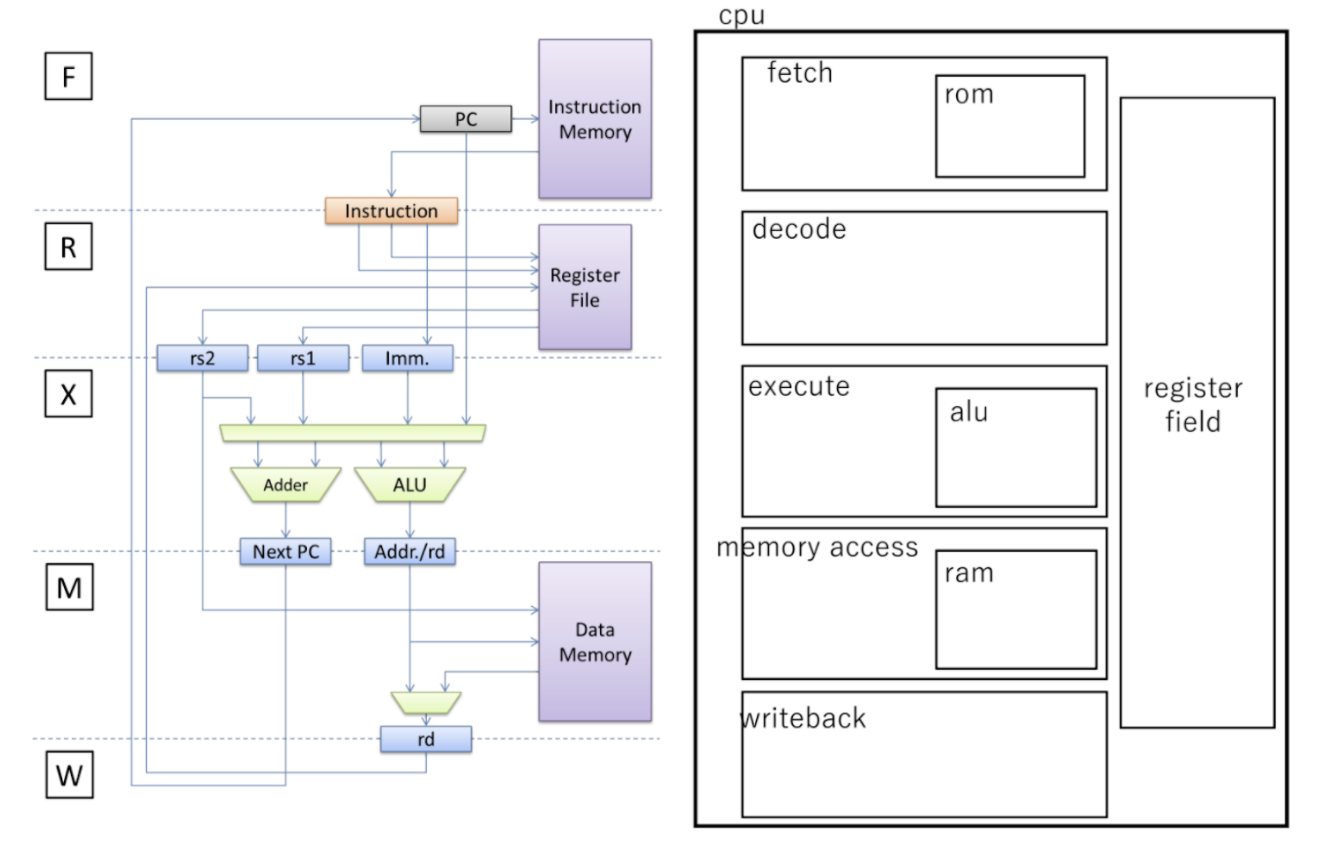
\includegraphics[width=0.5\textwidth]{2020-12-27-02-34-38.png}
 }
 \caption{参考にした図}
 \label{fig:}
\end{figure}


\subsection{作成したモジュール}
以下のようにwireを作成しそれぞれのモジュールへと繋げた。
\begin{itemize}
  \item fetch (romは内蔵)
  \item decoder
  \item execute
  \begin{itemize}
    \item alu
  \end{itemize}
  \item data\_mem
  \item reg\_file
  \item write\_back
  \item uart
  \item hardware\_counter
\end{itemize}

\subsection{cpuモジュールの実装}

% コード
\begin{lstlisting}[style={verilog-style}]
module cpu(
    input wire sysclk,
    input wire cpu_resetn,
    output wire uart_tx
    );
    wire rst;
    assign rst = cpu_resetn;

    wire [31:0] pc; //プログラムカウンタ
    wire [31:0] ir; //

    wire [4:0]  srcreg1_num;     
    wire [4:0]  srcreg2_num;     
    wire [4:0]  dstreg_num;    
    wire [31:0] imm;
    wire [5:0]	alucode;    
    wire [1:0]	aluop1_type; 
    wire [1:0]	aluop2_type;  
    wire	    reg_we;       
    wire	    is_load;     
    wire		is_store;    
    wire        is_halt;

    wire [31:0] srcreg1_data;
    wire [31:0] srcreg2_data;
    wire [31:0] nextpc;
    wire [31:0] alu_result;

    wire [31:0] dstreg_data;

    wire [31:0] ram_addr;

    //    wire [31:0] r_addr;
    wire [31:0] w_data;
    wire [31:0] r_data;

    wire [31:0] hc_OUT_data;

    // uart
    wire [7:0] uart_IN_data;
    wire uart_we;
    wire uart_OUT_data;\end{lstlisting}
    
    \subsubsection{モジュールの繋げ方}
    基本的に各モジュールをwireで繋いだだけ。
load 命令と計算結果のどちらかを使用するかだけはcpuモジュール内で決めた。
このようにした理由はis\_loadによってメモリ制御のモジュールの動作を変更するようにするより
cpuモジュール内でis\_loadによって繋げるwireを変更するように実装する方が楽だったからです。
\begin{lstlisting}[style={verilog-style}]
assign dstreg_data =  is_load   ?  r_data	: alu_result;
\end{lstlisting}


\section{苦労した点}
データのもろもろを理解できるのに二日間かかった。
fetch, reg\_file, data\_file をどのようにして作るか考えるのに時間がかかった。

\subsection{decoder作成(verilog文法の理解)}
\subsubsection{wireの値の変更}
srcreg1\_num, srcreg2\_num, dstreg\_num, imm の三つはwireのため
\begin{lstlisting}[style={verilog-style}]
  always @(ir) begin

  srcreg1_num <= ir[19:15];\end{lstlisting}

  のように値を変更するのは文法エラー
  alwaysの外側の位置でassign文で変更する必要がある。

  そこでop\_typeというレジスタを用意してその値をalways文ないで変更し、レジスタの値によってそれぞれのwireが接続する値を変更することにした。
\begin{lstlisting}[style={verilog-style}]
  reg [2:0] op_type;

  assign  srcreg1_num  = (op_type == `TYPE_U) ? 5'b0:
                         (op_type == `TYPE_J) ? 5'b0:
                         (op_type == `TYPE_I) ? ir[19:15]:
                         (op_type == `TYPE_B) ? ir[19:15]:
                         (op_type == `TYPE_S) ? ir[19:15]:
                         (op_type == `TYPE_R) ? ir[19:15]:
                         5'b0;   
  
  always @(ir) begin
      // 略
      op_type <= 3'd3;\end{lstlisting}


\subsubsection{wireの変更の時差}
以下コードないにうまく動くコードと動かないコードを入れる。
\begin{lstlisting}[style={verilog-style}]
  assign dstreg_num =   (op_type == `TYPE_U) ? ir[11:7]:
                        (op_type == `TYPE_J) ? ir[11:7]:
                        (op_type == `TYPE_I) ? ir[11:7]:
                        (op_type == `TYPE_B) ? 0:
                        (op_type == `TYPE_S) ? 0:
                        (op_type == `TYPE_R) ? ir[11:7]:
                        5'b0;
always @(ir) begin
// 略
`JAL   : begin
op_type <= `TYPE_J;

// うまくいかない
if (dstreg_num == 0) reg_we <= `REG_NONE;
else reg_we <= `REG_RD;

// うまくいく
if (ir[11:7] == 0) reg_we <= `DISABLE;
else reg_we <= `REG_RD;\end{lstlisting}
op\_type <= `TYPE\_J;とした直後にdstreg\_num=ir[11:7]となるわけではなく、時差があるため、レジスタではなく直接ir[11:7]を呼び出すことが必要。

\subsection{fetchの理解}
decoderとalu、executeを書いた後一番困ったのがfetchの理解でした。
与えられたbenchmarks/tests/ControlTransfer/code.hexから
どのように命令を読み取るのか、一番最初の初期値としてプログラムカウンタの値を
どのように設定すればいいのか分かりませんでした。
\subsubsection{fetch\_tb.vの作成}
fetchモジュールが機能しているのか確かめたかったため自前でfetch\_tb.vを作成しました。
これによりデータの取り出しが合っていることを確かめることができました。
個人的にalu,docoderのテストベンチの他にfetchのテストベンチも用意してくだされば
fetchの仕方をもう少し早く理解できたのではないかと思います。
\begin{lstlisting}[style={verilog-style}]
  `include "fetch.v"

  `define assertf(name, signal, value) \
          if (signal !== value) begin \
              $display("ASSERTION FAILED in %s : signal is '0x%x' but expected '0x%x'!", name, signal, value); \
              $finish; \
          end else begin \
              $display("    signal == value"); \
          end
  
  `define test_fetch(name, ex_ir) \
          $display("%s:", name); \
          `assertf("result", ir, ex_ir) \
          $display("%s test passed\n", name); \
  
  
  module fetch_tb;
      reg [31:0] pc;
      wire [31:0] ir;
  
  
      fetch fetch(
          .pc(pc)
          ,.ir(ir));
  
      initial begin
        pc = 32'h8000;
        $display("%d",pc);
        $display("%d",pc[31:2]);
        #10
  
          `test_fetch("fetch", 32'h0080006f)
          $display("all tests passed!");
      end
  
  endmodule
  
  \end{lstlisting}

  出力
  \begin{lstlisting}
[Running] fetch_tb.v
WARNING: ./fetch.v:6: $readmemh(/Users/momoka/git/microprocessor/benchmarks/tests/ControlTransfer/code.hex): Not enough words in the file for the requested range [0:32767].
ERROR: ./fetch.v:8: $readmemh: Unable to open /home/denjo/microprocessor/benchmarks/tests/Uart/code.hex for reading.
      32768
      8192
fetch:
    ir == 32'h0080006f
fetch test passed

all tests passed!
[Done] exit with code=0 in 0.192 seconds\end{lstlisting}
ここではファイルbenchmarks/tests/Uart/code.hex
の8193行目の内容が0080006fとなっているかを確かめるテストケースである。
結局8193行目の内容を得るためにはpc=32’h8000とすることが正解でした。

$pc = 32’h8000 = 2^{15} = 32768 = 4 \times 8192$

最初の命令は8193行目に出てくる。一命令32ビットだがメモリ空間はワードアドレッシングのため、$32\div8=4$
倍した値をpcにする必要がある。よってpcの値は$4 \times 8192$とするべき。

\subsection{data\_memモジュールの作成}
load,storeの知識があやふやだったためとても難したかった。
\subsubsection{loadの作成}
最初はstoreと同じようにクロック同期にしていたが、それだと
欲しい値がえられるのが1クロック後からになってしまうため
assign文で書くことにした。
シングルサイクルプロセッサなのでクロック同期はwrite\_backモジュールの
一箇所のみにした。
\begin{lstlisting}[style={verilog-style}]
assign r_data = (alucode == `ALU_LB  &&  addr[1:0] == 2'd0) ? {{24{ram[addr[16:2]][7]}}, ram[addr[16:2]][7:0]}:
                (alucode == `ALU_LB  &&  addr[1:0] == 2'd1) ? {{24{ram[addr[16:2]][15]}}, ram[addr[16:2]][15:8]}:
                (alucode == `ALU_LB  &&  addr[1:0] == 2'd2) ? {{24{ram[addr[16:2]][23]}}, ram[addr[16:2]][23:16]}:
                (alucode == `ALU_LB  &&  addr[1:0] == 2'd3) ? {{24{ram[addr[16:2]][31]}}, ram[addr[16:2]][31:24]}:

                (alucode == `ALU_LH  &&  addr[1:0] == 2'd0) ? {{16{ram[addr[16:2]][15]}}, ram[addr[16:2]][15:0]}:
                (alucode == `ALU_LH  &&  addr[1:0] == 2'd1) ? {{16{ram[addr[16:2]][23]}}, ram[addr[16:2]][23:8]}:
                (alucode == `ALU_LH  &&  addr[1:0] == 2'd2) ? {{16{ram[addr[16:2]][31]}}, ram[addr[16:2]][31:16]}:

                (alucode == `ALU_LW  &&  addr[1:0] == 2'd3) ? ram[addr[16:2]][31:0]:

                (alucode == `ALU_LBU  &&  addr[1:0] == 2'd0) ? {{24{1'b0}}, ram[addr[16:2]][7:0]}:
                (alucode == `ALU_LBU  &&  addr[1:0] == 2'd1) ? {{24{1'b0}}, ram[addr[16:2]][15:8]}:
                (alucode == `ALU_LBU  &&  addr[1:0] == 2'd2) ? {{24{1'b0}}, ram[addr[16:2]][23:16]}:
                (alucode == `ALU_LBU  &&  addr[1:0] == 2'd3) ? {{24{1'b0}}, ram[addr[16:2]][31:24]}:

                (alucode == `ALU_LHU  &&  addr[1:0] == 2'd0) ? {{16{1'b0}}, ram[addr[16:2]][15:0]}:
                (alucode == `ALU_LHU  &&  addr[1:0] == 2'd1) ? {{16{1'b0}}, ram[addr[16:2]][23:8]}:
                (alucode == `ALU_LHU  &&  addr[1:0] == 2'd2) ? {{16{1'b0}}, ram[addr[16:2]][31:16]}:

                ram[addr[16:2]][31:0]; //どれにも当てはまらなかったら困る。とりあえず`ALU_LWと同じにする。
\end{lstlisting}

\section{困ったこと}
\subsection{verilatorの使用}
使おうとしたがエラーによりコンパイルしてくれなかったため使えなかった。
たくさんのwarningで勉強にはなった。

よくわからなかったwarning達

<= はタイミングずれるから=にしろよwarning。
そうなのか疑問に思いながら<=を=に変更したが動かず。


メモリの大きさが違うと言われた。直した。メモリの大きさは間違ってても動いてしまうことがあることがわかった。
ここら辺を直してもcase文のcase足りないwarningが残りそれによりコンパイルしてくれなかった。
(case文warning残してもコンパイルしてくれるやろって思って別のところに原因があると思い諦めた。

\section{工夫したこと}
\subsection{gitの使用}
学科pcデコードを書くことになれていないためmacのVScodeでコードを書いて学科pcにgitで送ってUbuntuでVivadoを使うという方法をとった。
他の人と違いverilogでシミュレーションをしたいときは毎回macから学科pcへgitを用いてコードを送ったためcommitの回数は多くなった。
gitを多用したためuartが昨日まで動いていたのに今日なぜか動かない。みたいな時にコードを見返すことができた




\subsubsection{iverilogの使用}
微妙な差だが、個人的にvivadoよりiverilogの方が文法エラーがわかりやすかった。
おもにiverilogで些細な文法ミスなどを発見してからgitを使って学科pcに送り
vivadoで全体のシミュレーションをして構造的なミスを見つける。といった使い分けをしていた。
\subsubsection{iverilogの環境構築}

\begin{lstlisting}
  brew install icarus-verilog\end{lstlisting}
以下のコマンドでコンパイルできるらしい
\begin{lstlisting}
  iverilog -o [出力ファイル名] -s [トップモジュール名] [.vファイルの羅列]\end{lstlisting}
VSCode上では専用のエクステンションを使用することで実行した。
  https://github.com/leafvmaple/vscode-verilog

特にdecoder\_tb.v,alu\_tb.vを実行するときはVSCode上でテストした方が分かりやすかった。


\section{やりたかったこと}
\subsection{完成}
uartまでしか完成させることができず、性能評価は周波数を下げても何も出力されませんでした。最後まで完成させたかったです。
またパイプライン化やりたかった。

\subsection{aluの変更}
 今回aluはaluのテストベンチに剃って作成したが、個人的にテストベンチにそって作成した結果のaluモジュールとexecuteモジュールの仕事の分担に疑問があった。
さらなる変更として現在のaluの仕事をexecuteに移動させてaluは計算、シフトのみを行う純粋なaluとしてのモジュールに変えたいと思った。
具体的には以下のように5ビットの制御信号をexecuteから受け取りそれにより決められた動作をするようなaluを作成したいと思った。
\begin{figure}[H]
 \centering
 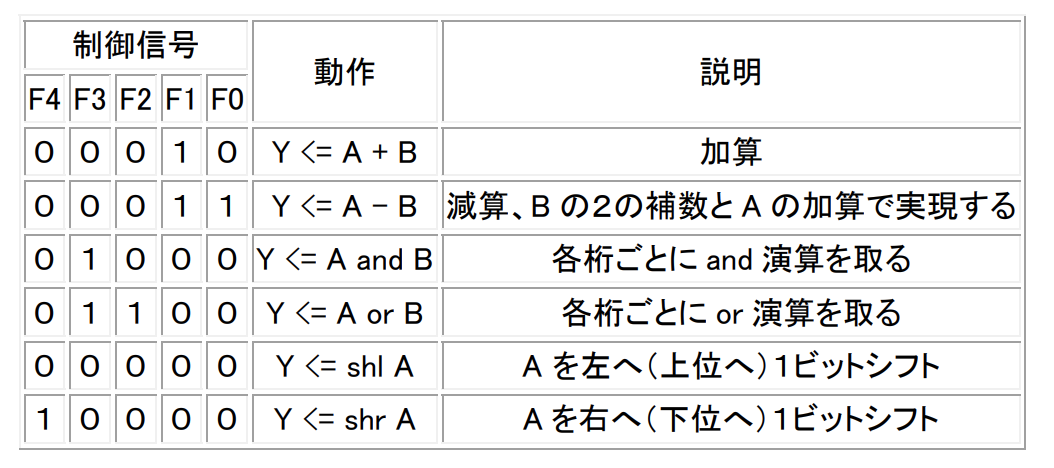
\includegraphics[width=0.5\textwidth]{2020-12-28-21-21-30.png}
 
 \caption{aluの制御信号と機能}
 \label{fig:}
\end{figure}

%----------------------------------------------------------------------------------------
%	参考文献
%----------------------------------------------------------------------------------------

\begin{thebibliography}{9}
    \bibitem{wiki} http://exp.mtl.t.u-tokyo.ac.jp/2020/b3exp/wikis/home
    \bibitem{kyokasho}実践 コンピュータアーキテクチャ(改訂版)





\end{thebibliography}
\end{document}
